\newcommand{\streamlinecomment}[1]{}

This chapter describes the \cgal\ 2D streamline placement package.
Basic definitions and notions are given in
Section~\ref{Section_2D_Streamlines_Definitions}.
Section~\ref{Section_2D_Streamlines_Fundamental_notions} gives a
description of the integration
process. Section~\ref{Section_2D_Streamlines_Strategy} provides a
brief description of the algorithm.
Section~\ref{Section_2D_Streamlines_Implementation} presents the
implementation of the package, and
Section~\ref{Section_2D_Streamlines_Example} details two example
placements.

\begin{figure}[ht!]
\begin{ccTexOnly}
\begin{center}
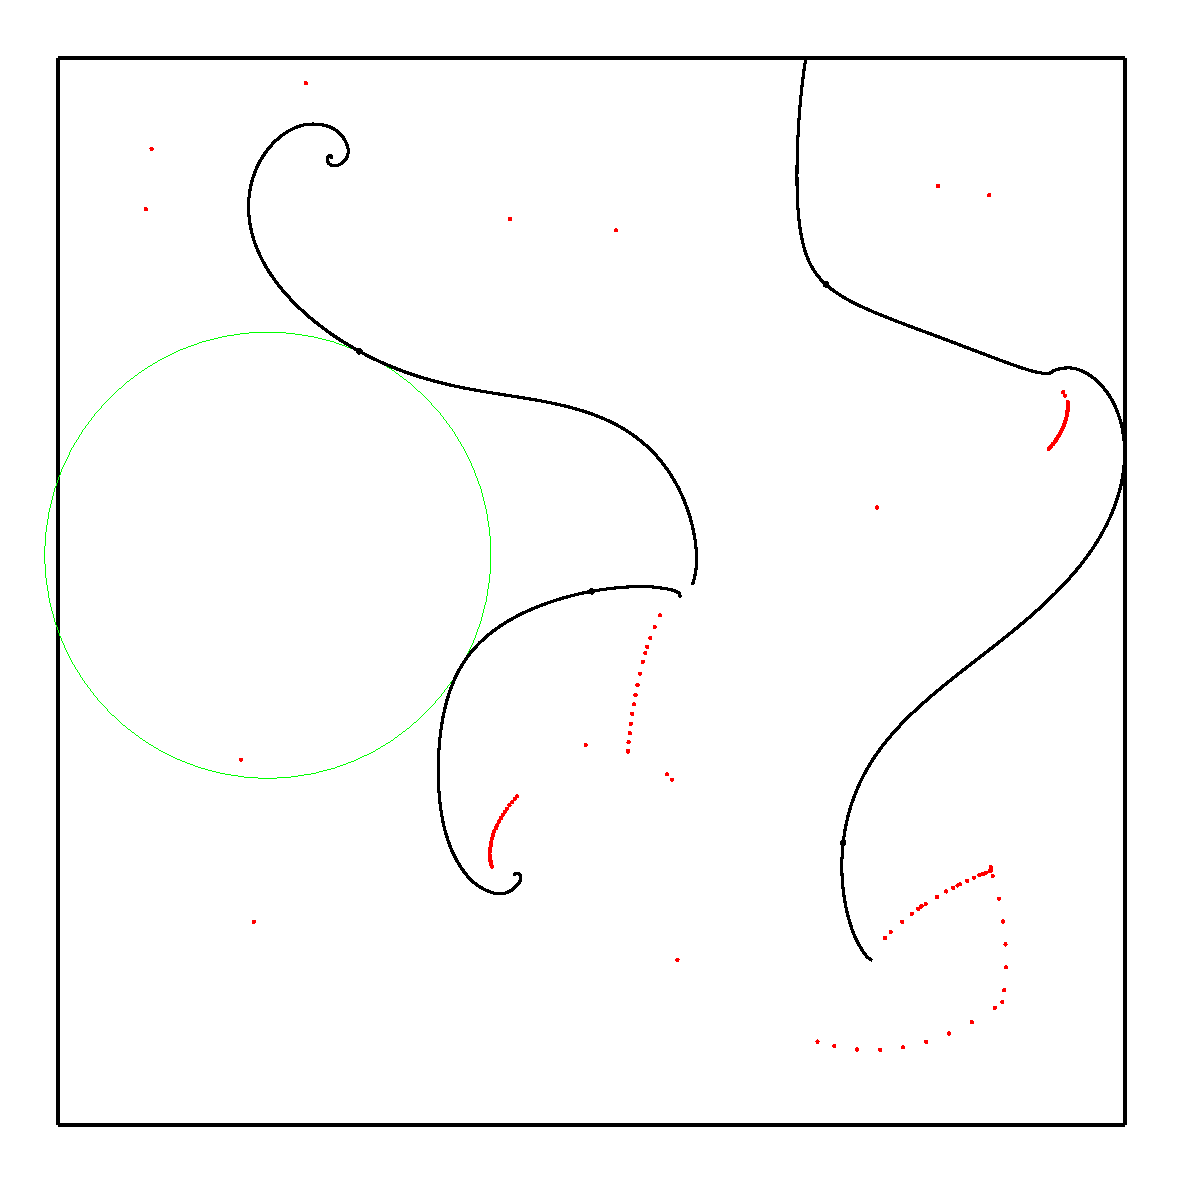
\includegraphics[width=4cm]{Stream_lines_2/1} \hspace*{0.5cm} 
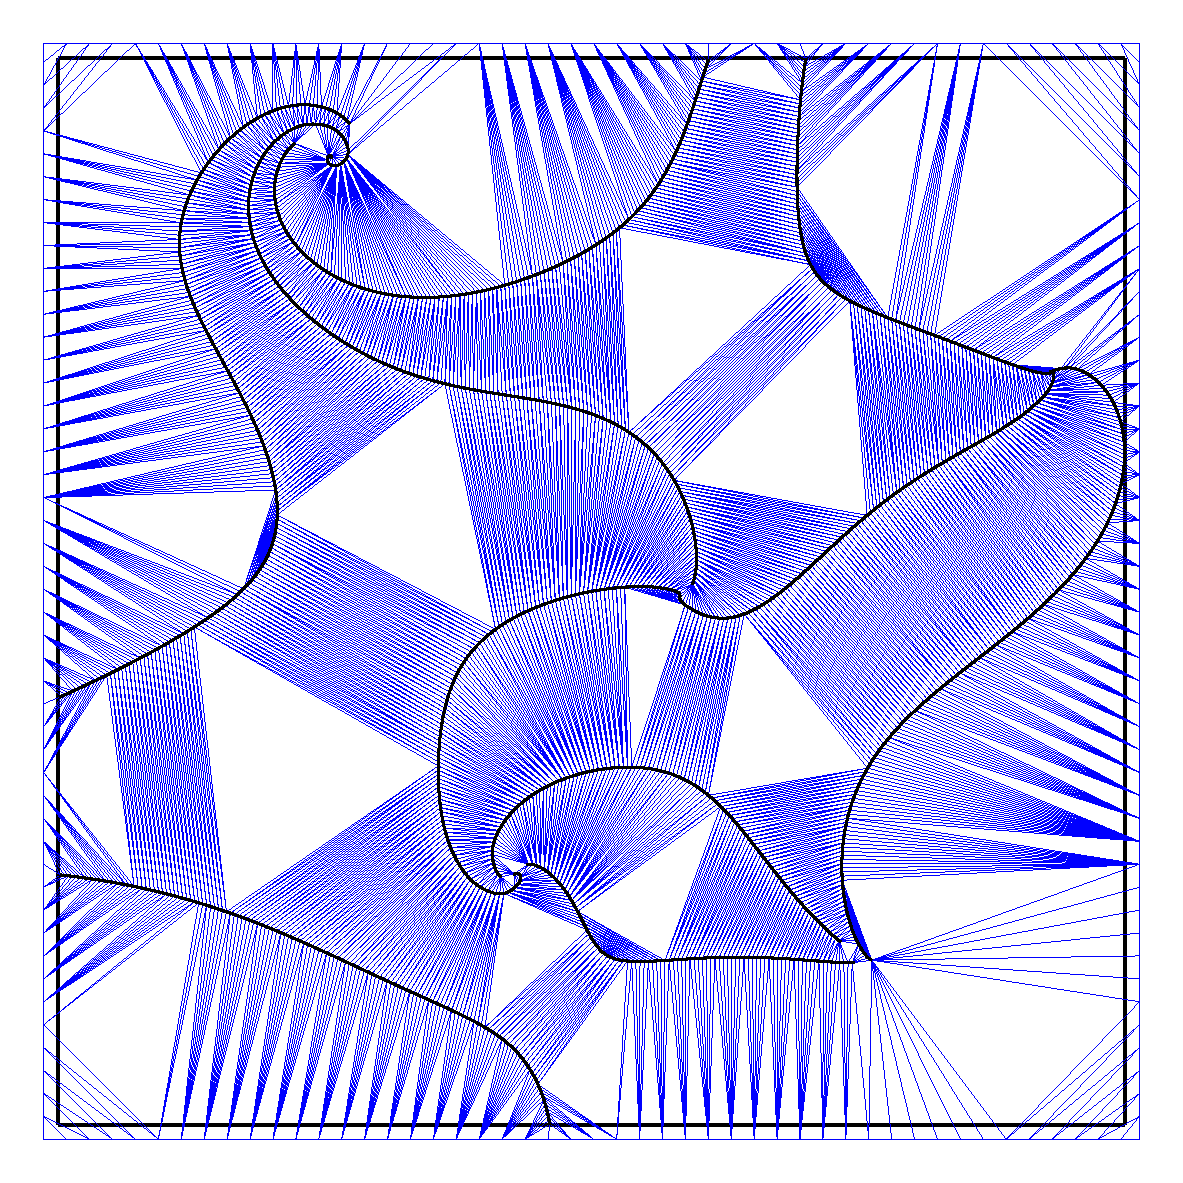
\includegraphics[width=4cm]{Stream_lines_2/2} \hspace*{0.5cm} 
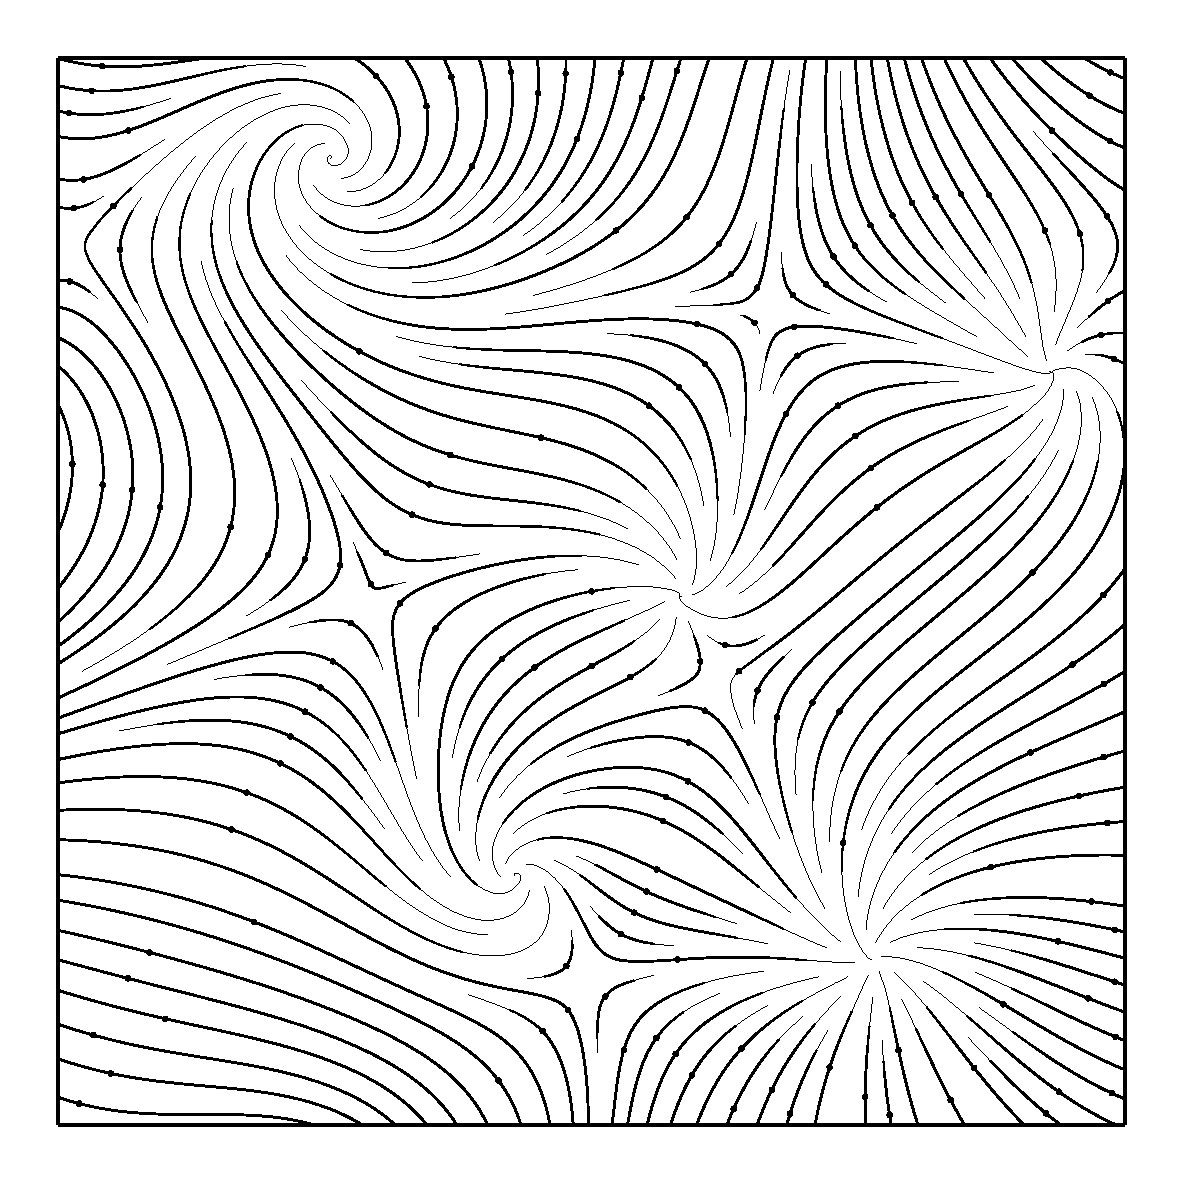
\includegraphics[width=4cm]{Stream_lines_2/3}
\end{center}
\end{ccTexOnly}

\label{illustration}
\begin{ccHtmlOnly}
<CENTER>
<img border=0 src="./1.gif" width=300>
<img border=0 src="./2.gif" width=300>
<img border=0 src="./3.gif" width=300>
</CENTER>
\end{ccHtmlOnly}
\begin{center}
\caption{The core idea of the algorithm is to integrate the
streamlines from the center of the biggest empty cavities in the
domain (left). A Delaunay triangulation of all the sample points is
used to model the streamlines and the spaces within the domain
(middle). A final result is shown (right).}
\end{center}
\end{figure}

\section{Definitions\label{Section_2D_Streamlines_Definitions}}

In physics, a \ccc{field} is an assignment of a quantity to every
point in space. For example, a gravitational field assigns a
gravitational potential to each point in space.\\

Vector and direction fields are commonly used for modeling physical
phenomena, where a direction and magnitude, namely a vector is assigned to
each point inside a domain (such as the magnitude and direction of the
force at each point in a magnetic field).\\

Streamlines are important tools for visualizing flow fields. A
\ccc{streamline} is a curve everywhere tangent to the field. In practice, 
a streamline is often represented as a polyline (series of points)
iteratively elongated by bidirectional numerical integration started
from a \ccc{seed point}, until it comes close to another streamline
(according to a specified distance called \ccc{the separating
distance}), hits the domain boundary, reaches a critical point or
generates a closed path.\\

A \ccc{valid} placement of streamlines consists of saturating the
domain with a set of tangential streamlines in accordance with a
specified \ccc{density}, determined by the \ccc{separating distance}
between the streamlines.

\section{Fundamental Notions\label{Section_2D_Streamlines_Fundamental_notions}}

A streamline can be considered as the path traced by an imaginary
massless particle dropped into a steady fluid flow described by the
field. The construction of this path consists in the solving an
ordinary differential equation for successive time intervals. In this
way, we obtain a series of points $p_k, 0<k<n$ which allow visualizing
the streamline. The differential equation is defined as follows :
$$\frac{dp}{dt} = v(p(t)), \ \ \ \ \ \ p(0) = p_0$$ where \ccc{p(t)} is the
position of the particle at time \ccc{t}, \ccc{v} is a function which
assigns a vector value at each point in the domain (possibly by
interpolation), and $p_0$ is the initial position.  The position after
a given interval $\Delta t$ is given by : $$p(t + \Delta t) = p(t) +
\int_t^{t+\Delta t} v(p(t)) dt$$. Several numeric methods have been
proposed to solve this equation. In this package, the Euler, and the
Second Order Runge-Kutta algorithm are implemented.

\subsection{Euler Integrator}

\begin{figure}[ht!]
\begin{ccTexOnly}
\begin{center}
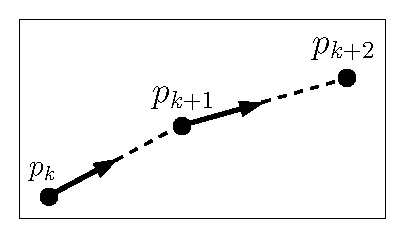
\includegraphics[width=4cm]{Stream_lines_2/euler_integrator}
\end{center}
\end{ccTexOnly}
\begin{ccHtmlOnly}
<CENTER>
<img border=0 src="./euler_integrator.gif" width=175>
</CENTER>
\end{ccHtmlOnly}
\begin{center}
\caption{Euler integrator.
\label{euler_fig}}
\end{center}
\end{figure}

This algorithm approximates the point computation by this formula
$$p_{k+1} = p_k + hv(p_k)$$ where \ccc{h} specifies the
\ccc{integration step} (see~Figure~\ref{euler_fig}). The integration
can be done forward (resp. backward) by specifying a positive
(resp. negative) integration step \ccc{h}. The streamline is then
constructed by successive integration from a seed point both forward
and backward.

\subsection{Second Order Runge-Kutta Integrator}

\begin{figure}[h!]
\begin{ccTexOnly}
\begin{center}
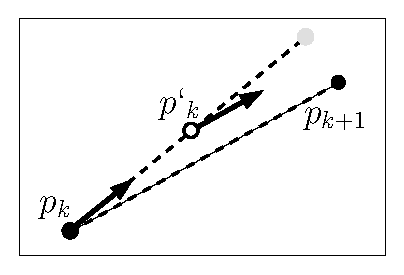
\includegraphics[width=4cm]{Stream_lines_2/runge_kutta_integrator}
\end{center}
\end{ccTexOnly}
\begin{ccHtmlOnly}
<CENTER>
<img border=0 src="./runge_kutta_integrator.gif" width=175>
</CENTER>
\end{ccHtmlOnly}
\begin{center}
\caption{Runge-Kutta second order integrator (The empty circle represents the intermediate point, and the gray disk represents the Euler integrated point).
\label{runge_kutta_fig}}
\end{center}
\end{figure}

This method introduces an intermediate point $p'_k$ between $p_k$ and $p_{k+1}$ to increase the
precision of the computation (see~Figure~\ref{runge_kutta_fig}), where:

$$
\begin{array}{ccccc}
    p'_k    & = & p_k & + & \frac{1}{2}hv(p_k) \\
    p_{k+1} & = & p_k & + & hv(p'_k)        \\
   \end{array}
$$

See~\cite{cgal:ptvf-nrcpp-02} for further details about numerical
integration.

\section{Farthest Point Seeding Strategy\label{Section_2D_Streamlines_Strategy}}

The algorithm implemented in this package~\cite{cgal:mad-fpsep-05}
consists of placing one streamline at a time by numerical integration
starting farthest away from all previously placed
streamlines.\\

The input of our algorithm is given by (i) a flow field, (ii) a
\textit{density} specified either globally, by the inverse of the
ideal spacing distance, or locally by a density field, and (iii) a
\textit{saturation} ratio over the desired spacing required to trigger
the seeding of a new streamline.\\


The input flow field is given by a discrete set of vectors or
directions sampled within a domain, associated with an interpolation
scheme (\textit{e.g.} bilinear interpolation over a regular grid, or
natural neighbor interpolation over an irregular point set to allow
for an evaluation at each point coordinate within the domain).\\

The \textit{output} is a streamline placement, represented as a list
of streamlines.  The core idea of our algorithm consists of placing
one streamline at a time by numerical integration seeded at the
farthest point from all previously placed streamlines.\\


The streamlines are approximated by polylines, whose points are
inserted to a 2D Delaunay
triangulation~(see~figure~\ref{illustration}). The empty circumscribed
circles of the Delaunay triangles provide us with a good approximation
of the cavities in the domain.\\

After each streamline integration, all incident triangles whose
circumcircle diameter is larger (within the saturation ratio) than the
desired spacing distance are pushed to a priority queue sorted by the
triangle circumcircle diameter. To start each new streamline
integration, the triangle with largest circumcircle diameter (and
hence the biggest cavity) is popped out of the queue. We first test if
it is still a valid triangle of the triangulation, since it could have
been destroyed by a streamline previously added to the
triangulation. If it is not, we pop another triangle out of the
queue. If it is, we use the center of its circumcircle as seed point
to integrate a new streamline.\\

Our algorithm terminates when the priority queue is empty. The size of
the biggest cavity being monotonically decreasing, our algorithm
guarantees the domain saturation.

\section{Implementation\label{Section_2D_Streamlines_Implementation}}

Streamlines are represented as polylines, and are obtained by
iterative integration from the seed point. A polyline is represented as a range of points. The computation is
processed via a list of Delaunay triangulation vertices.\\

To implement the triangular grid, the \cgal\
\ccc{Delaunay_triangulation_2} class is used. The priority queue used
to store candidate seed points is taken from the Standard Template
Library~\cite{cgal:sgcsi-stlpg-97}.

\section{Examples\label{Section_2D_Streamlines_Example}}

The first example illustrates the generation of a 2D streamline
placement from a vector field defined on a regular grid.
\ccIncludeExampleCode{Stream_lines_2/stl_regular_field.cpp}
The second example depicts the generation of a streamline placement from a vector
field defined on a triangular grid.
\ccIncludeExampleCode{Stream_lines_2/stl_triangular_field.cpp}
